\achapter{30}{Using the Singular Value Decomposition} \label{sec:pseudoinverses}

\vspace*{-17 pt}
\framebox{
\parbox{\dimexpr\linewidth-3\fboxsep-3\fboxrule}
{\begin{fqs}
\item What is the condition number of a matrix and what does it tell us about the matrix? 
\item What is the pseudoinverse of a matrix? 
\item Why are pseudoinverses useful? 
%\item How can we find a least squares solution to an equation $A \vx = \vb$? 
\item How does the pseudoinverse of a matrix allow us to find least squares solutions to linear systems?
\end{fqs}}}% \hspace*{3 pt}}

\vspace*{13 pt}

\csection{Application: Global Positioning System}      

You are probably familiar with the Global Positioning System (GPS). The system allows anyone with the appropriate software to accurately determine their location at any time. The applications are almost endless, including getting real-time driving directions while in your car, guiding missiles, and providing distances on golf courses. 

The GPS is a worldwide radio-navigation system owned by the US government and operated by the US Air Force. GPS is one of four global navigation satellite systems. At least twenty four GPS satellites orbit the Earth at an altitude of approximately 11,000 nautical miles. The satellites are placed so that at any time at least four of them can be accessed by a GPS receiver. Each satellite carries an atomic clock to relay a time stamp along with its position in space. There are five ground stations to coordinate and ensure that the system is working properly. 

The system works by triangulation, but there is also error involved in the measurements that go into determining position. Later in this section we will see how the method of least squares can be used to determine the receiver's position.


\csection{Introduction} A singular value decomposition has many applications, and in this section we discuss how a singular value decomposition can be used in image compression, to determine how sensitive a matrix can be to rounding errors in the process of row reduction, and to solve least squares problems.  


\csection{Image Compression}

The digital age has brought many new opportunities for the collection, analysis, and dissemination of information. Along with these opportunities come new difficulties as well. All of this digital information must be stored in some way and be retrievable in an efficient manner. A singular value decomposition of digitally stored information can be used to compress the information or clean up corrupted information. In this section we will see how a singular value decomposition can be used in image compression. While a singular value decomposition is normally used with very large matrices, we will restrict ourselves to small examples so that we can more clearly see how a singular value decomposition is applied.

\begin{pa} \label{pa:7_d_1} Let $A = \frac{1}{4}\left[ \begin{array}{ccrr} 67&29&-31&-73 \\ 29&67&-73&-31 \\ 31&73&-67&-29  \\ 73&31&-29&-67 \end{array} \right]$. A singular value decomposition for $A$ is $U \Sigma V^{\tr}$, where
\begin{align*}
U &= [\vu_1 \ \vu_2 \ \vu_3 \ \vu_4] = \frac{1}{2} \left[ \begin{array}{crrr} 1&-1&1&-1\\1&1&1&1\\1&1&-1&-1\\1&-1&-1&1 \end{array} \right], \\
 \Sigma &=  \left[ \begin{array}{cccc} 50&0&0&0\\0&20&0&0\\0&0&2&0\\0&0&0&1 \end{array} \right], \\
 V &= [\vv_1 \ \vv_2 \ \vv_3 \ \vv_4] = \frac{1}{2} \left[ \begin{array}{rrrr} 1&1&-1&1\\1&-1&-1&-1\\-1&1&-1&-1\\-1&-1&-1&1 \end{array} \right].
 \end{align*}
	\be
	\item Write the summands in the corresponding outer product decomposition of $A$.
	
	\item The outer product decomposition of $A$ writes $A$ as a sum of rank 1 matrices (the summands $\sigma_i \vu_i \vv_i^{\tr})$. Each summand contains some information about the matrix $A$. Since $\sigma_1$ is the largest of the singular values, it is reasonable to expect that the summand $A_1 = \sigma_1 \vu_1  \vv_1^{\tr}$ contains the most information about $A$ among all of the summands. To get a measure of how much information $A_1$ contains of $A$, we can think of $A$ as simply a long vector in $\R^{mn}$ where we have folded the data into a rectangular array (we will see later why taking the norm as the norm of the vector in $\R^{nm}$ makes sense, but for now, just use this definition). If we are interested in determining the error in approximating an image by a compressed image, it makes sense to use the standard norm in $\R^{mn}$ to determine length and distance, which is really just the Frobenius norm that comes from the Frobenius inner product defined by
\begin{equation} \label{eq:7_d_Frobenius_ip}
\langle U,V \rangle = \sum u_{ij}v_{ij},
\end{equation}
where $U = [u_{ij}]$ and $V = [v_{ij}]$ are $m \times n$ matrices. (That (\ref{eq:7_d_Frobenius_ip}) defines an inner product on the set of all $n \times n$ matrices is left to discuss in a later section.) So in this section all the norms for matrices will refer to the Frobenius norm. Rather than computing the distance between $A_1$ and $A$ to measure the error, we are more interested in the relative error
\[\frac{||A-A_1||}{||A||}.\]
	\ba
	\item Calculate the relative error in approximating $A$ by $A_1$. What does this tell us about how much information $A_1$ contains about $A$? 
	
	\item Let $A_2 = \sum_{k=1}^2 \sigma_k \vu_k \vv_k^{\tr}$. Calculate the relative error in approximating $A$ by $A_2$. What does this tell us about how much information $A_2$ contains about $A$? 
	

	\item Let $A_3 =  \sum_{k=1}^3 \sigma_k \vu_k \vv_k^{\tr}$. Calculate the relative error in approximating $A$ by $A_3$. What does this tell us about how much information $A_3$ contains about $A$? 
	
	\item Let $A_4 =  \sum_{k=1}^4 \sigma_k \vu_k \vv_k^{\tr}$. Calculate the relative error in approximating $A$ by $A_4$. What does this tell us about how much information $A_4$ contains about $A$? Why?

		\ea
	\ee
\end{pa}

The first step in compressing an image is to digitize the image. There are many ways to do this and we will consider one of the simplest ways and only work with gray-scale images, with the scale from 0 (black) to 255 (white).  A digital image can be created by taking a small grid of squares (called pixels) and coloring each pixel with some shade of gray.  The resolution of this grid is a measure of how many pixels are used per square inch.  As an example,  consider the 16 by 16 pixel picture of a flower shown in Figure \ref{Fig:7_c_Flower}.
\begin{figure}[h]
\begin{center}
\resizebox{!}{2.5in}{\includegraphics{7_c_Flower}}
\end{center}
\caption{A 16 by 16 pixel image}
\label{Fig:7_c_Flower}
\end{figure}

To store this image pixel by pixel would require $16 \times 16 = 256$ units of storage space (1 for each pixel). If we let $M$ be the matrix whose $i,j$th entry is the scale of the $i,j$th pixel, then $M$ is the matrix 
%\[ \left[ \begin {array}{cccccccccccccccc} 240&240&240&240&130&130&240&
%130&130&240&240&240&240&240&240&240\\ 240&240&240&
%130&175&175&130&175&175&130&240&240&240&240&240&240
%\\ 240&240&130&130&175&175&130&175&175&130&130&240&
%240&240&240&240\\ 240&130&175&175&130&175&175&175&
%130&175&175&130&240&240&240&240\\ 240&240&130&175&
%175&130&175&130&175&175&130&240&240&240&240&240\\ 
%255&240&240&130&130&175&175&175&130&130&240&240&225&240&240&240
%\\ 240&240&130&175&175&130&130&130&175&175&130&240&
%225&255&240&240\\ 240&240&130&175&130&240&130&240&
%130&175&130&240&255&255&255&240\\ 240&240&240&130&
%240&240&75&240&240&130&240&255&255&255&255&255\\ \noalign{\medskip}240
%&240&240&240&240&240&75&240&240&240&240&240&240&240&240&240
%\\ 240&240&240&75&75&240&75&240&75&75&240&240&240&
%240&240&240\\ 50&240&240&240&75&240&75&240&75&240&
%240&240&240&50&240&240\\ 240&75&240&240&240&75&75&75
%&240&240&50&240&50&240&240&50\\ 240&240&75&240&240&
%240&75&240&240&50&240&50&240&240&50&240\\ 75&75&75&
%75&75&75&75&75&75&75&75&75&75&75&75&75\\ 75&75&75&75
%&75&75&75&75&75&75&75&75&75&75&75&75\end {array} \right].\]

\[\tiny{ \left[ \begin{array}{cccccccccccccccc} 240&240&240&240&130&130&240&
130&130&240&240&240&240&240&240&240\\ 240&240&240&
130&175&175&130&175&175&130&240&240&240&240&240&240
\\ 240&240&130&130&175&175&130&175&175&130&130&240&
240&240&240&240\\ 240&130&175&175&130&175&175&175&
130&175&175&130&240&240&240&240\\ 240&240&130&175&
175&130&175&130&175&175&130&240&240&240&240&240\\ 
255&240&240&130&130&175&175&175&130&130&240&240&225&240&240&240
\\ 240&240&130&175&175&130&130&130&175&175&130&240&
225&255&240&240\\ 240&240&130&175&130&240&130&240&
130&175&130&240&255&255&255&240\\ 240&240&240&130&
240&240&75&240&240&130&240&255&255&255&255&255\\ 240
&240&240&240&240&240&75&240&240&240&240&240&240&240&240&240
\\ 240&240&240&75&75&240&75&240&75&75&240&240&240&
240&240&240\\ 50&240&240&240&75&240&75&240&75&240&
240&240&240&50&240&240\\ 240&75&240&240&240&75&75&75
&240&240&50&240&50&240&240&50\\ 240&240&75&240&240&
240&75&240&240&50&240&50&240&240&50&240\\ 75&75&75&
75&75&75&75&75&75&75&75&75&75&75&75&75\\ 75&75&75&75
&75&75&75&75&75&75&75&75&75&75&75&75 \end{array} \right]}.\]



Recall that if $U \Sigma V^{\tr}$ is a singular value decomposition for $M$, then we can also write $M$ in the form
\[M=\sigma_1 \vu_1\vv_1^{\tr} + \sigma_2 \vu_2\vv_2^{\tr} + \sigma_3 \vu_3\vv_3^{\tr} + \cdots + \sigma_{16} \vu_{16}\vv_{16}^{\tr}.\]
given in (\ref{eq:7_c_SVD}). For this $M$, the singular values are approximately
\begin{equation} \left[ \begin {array}{c}  3006.770088367795 \\ 439.13109000200205 \\ 382.1756550649652 \\ 312.1181752764884 \\ 254.45105800344953 \\ 203.36470770057494 \\ 152.8696215072527 \\ 101.29084240890717 \\ 63.80803769229468 \\ 39.6189181773536 \\ 17.091891798245463 \\ 12.304589419140656 \\ 4.729898943556077 \\ 2.828719409809012 \\ 6.94442317024232 \times 10^{-15} \\2.19689952047833 \times 10^{-15} \end {array} \right]. \label{eq:7_c_Flower_sing_values}
\end{equation}

Notice that some of these singular values are very small compared to others. As in Preview Activity \ref{pa:7_d_1}, the terms with the largest singular values contain most of the information about the matrix.  Thus, we shouldn't lose much information if we eliminate the small singular values. In this particular example, the last 4 singular values are significantly smaller than the rest. If we let
\[M_{12} = \sigma_1 \vu_1\vv_1^{\tr} + \sigma_2 \vu_2\vv_2^{\tr} + \sigma_3 \vu_3\vv_3^{\tr} + \cdots + \sigma_{12} \vu_{12}\vv_{12}^{\tr},\]
then we should expect the image determined by $M_{12}$ to be close to the image made by $M$. The two images are presented side by side in Figure \ref{F:7_c_Compress}.
\begin{figure}[h]
\begin{center}
\resizebox{!}{2.0in}{\includegraphics{7_c_Flower}} \hspace{0.5in} \resizebox{!}{2.0in}{
\includegraphics{7_c_CFlower}}
\end{center}
\caption{{\scriptsize A 16 by 16 pixel image and a compressed image using a singular value decomposition.}}
\label{F:7_c_Compress}
\end{figure}

This small example illustrates the general idea. Suppose we had a satellite image that was $1000 \times 1000$ pixels and we let $M$ represent this image. If we have a singular value decomposition of this image $M$, say
\[M = \sigma_1 \vu_1\vv_1^{\tr} + \sigma_2 \vu_2\vv_2^{\tr} + \sigma_3 \vu_3\vv_3^{\tr} + \cdots + \sigma_{r} \vu_{r}\vv_{r}^{\tr},\]
if the rank of $M$ is large, it is likely that many of the singular values will be very small. If we only keep $s$ of the singular values, we can approximate $M$ by
\[M_s = \sigma_1 \vu_1\vv_1^{\tr} + \sigma_2 \vu_2\vv_2^{\tr} + \sigma_3 \vu_3\vv_3^{\tr} + \cdots + \sigma_{s} \vu_{s}\vv_{s}^{\tr}\]
and store the image with only the vectors $\sigma_1 \vu_1$, $\sigma_2 \vu_2$, $\ldots$, $\sigma_{s}\vu_s$, $\vv_1$, $\vv_1$, $\ldots$, $\vv_s$.
For example, if we only need 10 of the singular values of a satellite image ($s = 10$), then we can store the satellite image with only 20 vectors in $\R^{1000}$ or with $20 \times 1000 = 20,000$ numbers instead of $1000 \times 1000 = 1,000,000$ numbers.

A similar process can be used to denoise data.\footnote{For example, as stated in \url{http://www2.imm.dtu.dk/~pch/Projekter/tsvd.html}, ``The SVD [singular value decomposition] has also applications in digital signal processing, e.g., as a method for noise reduction. The central idea is to let a matrix $A$ represent the noisy signal, compute the SVD, and then discard small singular values of $A$. It can be shown that the small singular values mainly represent the noise, and thus the rank-$k$ matrix $A_k$ represents a filtered signal with less noise."}

\csection{Calculating the Error in Approximating an Image}

In the context where a matrix represents an image, the operator aspect of the matrix is irrelevant -- we are only interested in the matrix as a holder of information. In this situation, we think of an $m \times n$ matrix as simply a long vector in $\R^{mn}$ where we have folded the data into a rectangular array. If we are interested in determining the error in approximating an image by a compressed image, it makes sense to use the standard norm in $\R^{mn}$ to determine length and distance. This leads to what is called the \emph{Frobenius} norm of a matrix. The Frobenius norm $||M||_F$ of an $m \times n$ matrix $M = [m_{ij}]$ is
\[||M||_F = \sqrt{ \sum m_{ij}^2 }.\]
There is a natural corresponding inner product on the set of $m \times n$ matrices (called the \emph{Frobenius product}) defined by
\[\langle A,B \rangle = \sum a_{ij}b_{ij},\]
where $A = [a_{ij}]$ and $B = [b_{ij}]$ are $m \times n$ matrices.%\footnote{This is the same inner product that we defined as the Frobenius inner product in Section \ref{sec:inner_products}, where $\langle A, B \rangle = \trace\left(AB^{\tr}\right)$.}
Note that
\[||A||_F = \sqrt{\langle A, A\rangle}.\]

If an $m \times n$ matrix $M$ of rank $r$ has a singular value decomposition $M = U \Sigma V^{\tr}$, we have seen that we can write $M$ as an outer product
\begin{equation}
M = \sigma_1 \vu_1\vv_1^{\tr} + \sigma_2 \vu_2\vv_2^{\tr} + \sigma_3 \vu_3\vv_3^{\tr} + \cdots + \sigma_{r} \vu_{r}\vv_{r}^{\tr}, \label{eq:7_c_outer_product}
\end{equation}
where the $\vu_i$ are the columns of $U$ and the $\vv_j$ the columns of $V$. Each of the products $\vu_i \vv_i^{\tr}$ is an $m \times n$ matrix. Since the columns of $\vu_i \vv_i^{\tr}$ are all scalar multiples of $\vu_i$, the matrix $\vu_i \vv_i^{\tr}$ is a rank 1 matrix. So (\ref{eq:7_c_outer_product}) expresses $M$ as a sum of rank 1 matrices. Moreover, if we let $\vx$ and $\vw$ be $m \times 1$ vectors and let $\vy$ and $\vz$ be $n \times 1$ vectors with $\vy = [y_1 \ y_2 \ \ldots \ y_n]^{\tr}$ and $\vz = [z_1 \ z_2 \ \ldots \ z_n]^{\tr}$, then
\begin{align*}
\langle \vx\vy^{\tr}, \vw\vz^{\tr} \rangle &= \langle [y_1\vx \ y_2\vx \ \cdots \ y_n\vx], [z_1\vw \ z_2\vw \ \cdots \ z_n\vw] \rangle \\
	&= \sum (y_i\vx) \cdot (z_i\vw) \\
	&= \sum (y_iz_i)(\vx \cdot \vw) \\
	&= (\vx \cdot \vw) \sum (y_iz_i) \\
	&= (\vx \cdot \vw) (\vy \cdot \vz).
\end{align*}

Using the vectors from the singular value decomposition of $M$ as in (\ref{eq:7_c_outer_product}) we see that
\[\langle \vu_i\vv_i^{\tr}, \vu_j\vv_j^{\tr} \rangle = (\vu_i \cdot \vu_j)(\vv_i \cdot \vv_j) = \begin{cases}
0, &\text{ if } i\neq j, \\
1, &\text{ if } i = j.
\end{cases}\]
It follows that
\begin{equation}
||M||_F^2 = \sum \sigma_i^2 (\vu_i \cdot \vu_i)(\vv_i \cdot \vv_i) = \sum \sigma_i^2. \label{eq:7_c_SVD_norm}
\end{equation}



\begin{activity} Verify (\ref{eq:7_c_SVD_norm}) that $||M||_F^2 = \sum \sigma_i^2$.



\end{activity}

When we used the singular value decomposition to approximate the image defined by $M$, we replaced $M$ with a matrix of the form
\begin{equation}
M_k = \sigma_1 \vu_1\vv_1^{\tr} + \sigma_2 \vu_2\vv_2^{\tr} + \sigma_3 \vu_3\vv_3^{\tr} + \cdots + \sigma_{k} \vu_{k}\vv_{k}^{\tr}. \label{eq:7_c_outer_product_k}
\end{equation}
We call $M_k$ the rank $k$ approximation to $M$. Notice that the outer product expansion in (\ref{eq:7_c_outer_product_k}) is in fact a singular value decomposition for $M_k$. The error $E_k$ in approximating $M$ with $M_k$ is
\begin{equation}
E_k = M - M_k = \sigma_{k+1} \vu_{k+1}\vv_{k+1}^{\tr} + \sigma_{k+2} \vu_{k+2}\vv_{k+2}^{\tr} + \cdots + \sigma_{r} \vu_{r}\vv_{r}^{\tr}. \label{eq:7_c_outer_product_error}
\end{equation}
Once again, notice that (\ref{eq:7_c_outer_product_error}) is a singular value decomposition for $E_k$. We define the relative error in approximating $M$ with $M_k$ as
\[\ds \frac{||E_k||}{||M||}.\]
Now (\ref{eq:7_c_SVD_norm}) shows that
\[\ds \frac{||E_k||}{||M||} = \sqrt{ \frac{\sum_{i=k+1}^r \sigma_i^2}{\sum_{i=1}^r \sigma_i^2} }.\]
In applications, we often want to retain a certain degree of accuracy in our approximations and this error term can help us accomplish that.

In our flower example, the singular values of $M$ are given in (\ref{eq:7_c_Flower_sing_values}). The relative error in approximating $M$ with $M_{12}$ is
\[\sqrt{ \frac{\sum_{i=13}^{16} \sigma_i^2}{\sum_{i=1}^{16} \sigma_i^2} } \approx 0.0018.\]
Errors (rounded to 4 decimal places) for approximating $M$ with some of the $M_k$ are shown in Table \ref{T:7_c_Errors}
\begin{table}[h]
\begin{center}
\begin{tabular}{|c|c|c|c|c|c|} \hline
$k$	&10 & 9 & 8 & 7 & 6  \\ \hline
$\frac{||E_k||}{||M||}$ &0.0070 &0.0146 &0.0252 &0.0413 &0.06426 \\ \hline
\end{tabular} \vspace{4pt}
\begin{tabular}{|c|c|c|c|c|c|} \hline
$k$	&5 & 4 &3 & 2 & 1  \\ \hline
$\frac{||E_k||}{||M||}$ &0.0918 &0.1231 &0.1590 &0.201 &0.2460 \\ \hline
\end{tabular}
\caption{ Errors in approximating $M$ by $M_k$}
\label{T:7_c_Errors}
\end{center}
\end{table}



\begin{activity} Let $M$ represent the flower image.
	\ba
	\item Find the relative errors in approximating $M$ by $M_{13}$ and $M_{14}$. You may use the fact that  $\sqrt{\sum_{i=1}^{16} \sigma_i^2} \approx 3102.0679$.



	\item About how much of the information in the image is contained in the rank 1 approximation? Explain.
	
	
	
	\ea
\end{activity}


\csection{The Condition Number of a Matrix}

A singular value decomposition for a matrix $A$ can tell us a lot about how difficult it is to accurately solve a system $A \vx = \vb$. Solutions to systems of linear equations can be very sensitive to rounding as the next exercise demonstrates.



\begin{activity} \label{act:7_c_cond_num} Find the solution to each of the systems.
	\ba
	\item $\left[ \begin{array}{cc} 1.0000&1.0000 \\ 1.0000&1.0005 \end{array} \right] \left[ \begin{array}{c} x \\ y \end{array} \right] = \left[ \begin{array}{c} 2.0000 \\ 2.0050 \end{array} \right]$
	
	
	
	\item $\left[ \begin{array}{cc} 1.000&1.000 \\ 1.000&1.001 \end{array} \right] \left[ \begin{array}{c} x \\ y \end{array} \right] = \left[ \begin{array}{c} 2.000 \\ 2.005 \end{array} \right]$

	
	
	\ea
\end{activity}

Notice that a simple rounding in the $(2,2)$ entry of the coefficient matrix led to a significantly different solution. If there are rounding errors at any stage of the Gaussian elimination process, they can be compounded by further row operations. This is an important problem since computers can only approximate irrational numbers with rational numbers and so rounding can be critical. Finding ways of dealing with these kinds of errors is an area of on-going research in numerical linear algebra. This problem is given a name.

\begin{definition} A matrix $A$ is \textbf{ill-conditioned} if relatively small changes in any entries of $A$ can produce significant changes in solutions to the system $A\vx = \vb$.
\end{definition}

A matrix that is not ill-conditioned is said to be \emph{well-conditioned}. Since small changes in entries of ill-conditioned matrices can lead to large errors in computations, it is an important problem in linear algebra to have a way to measure how ill-conditioned a matrix is. This idea will ultimately lead us to the condition number of a matrix.

Suppose we want to solve the system $A \vx = \vb$, where $A$ is an invertible matrix. Activity \ref{act:7_c_cond_num} illustrates that if $A$ is really close to being singular, then small changes in the entries of $A$ can have significant effects on the solution to the system. So the system can be very hard to solve accurately if $A$ is close to singular. It is important to have a sense of how ``good" we can expect any calculated solution to be. Suppose we think we solve the system $A \vx = \vb$ but, through rounding error in our calculation of $A$, get a solution $\vx'$ so that $A \vx' = \vb'$, where $\vb'$ is not exactly $\vb$. Let $\Delta \vx$ be the error in our calculated solution and $\Delta \vb$ the difference between $\vb'$ and $\vb$. We would like to know how large the error $||\Delta \vx||$ can be. But this isn't exactly the right question. We could scale everything to make $||\Delta \vx||$ as large as we want. What we really need is a measure of the \emph{relative error} $\frac{||\Delta \vx||}{||\vx||}$, or how big the error is compared to $||\vx||$ itself. More specifically, we want to know how large the relative error in $\Delta \vx$ is compared to the relative error in $\Delta \vb$. In other words, we want to know how good the relative error in $\Delta \vb$ is as a predictor of the relative error in $\Delta \vx$ (we may have some control over the relative error in $\Delta \vb$, perhaps by keeping more significant digits). So we want know if there is a best constant $C$ such that
\[\frac{||\Delta \vx||}{||\vx||} \leq C \frac{||\Delta \vb||}{||\vb||}.\]
This best constant $C$ is the condition number -- a measure of how well the relative error in $\Delta \vb$ predicts the relative error in $\Delta \vx$. How can we find $C$?

Since $A \vx' = \vb'$ we have
\begin{equation*}
A(\vx + \Delta \vx) = \vb + \Delta \vb.
\end{equation*}
Distributing on the left and using the fact that $A\vx = \vb$ gives us
\begin{equation*}
A\Delta \vx = \Delta \vb. \label{eq:7_c_cn}
\end{equation*}

We return for a moment to the operator norm of a matrix. This is an appropriate norm to use here since we are considering $A$ to be a transformation. Recall that if $A$ is an $m \times n$ matrix, we defined the operator norm of $A$ to be
\[||A|| = \max_{||\vx|| \neq \vzero} \left\{\frac{||A\vx||}{||\vx||} \right\} = \max_{||\vx||=1} \{||A\vx||\}.\]
One important property that the norm has is that if the product $AB$ is defined, then
\[||AB|| \leq ||A|| \ ||B||.\]
To see why, notice that
\[\frac{||AB\vx||}{||\vx||} = \frac{||A(B\vx)||}{||B\vx||} \ \frac{||B\vx||}{||\vx||}.\]
Now $\frac{||A(B\vx)||}{||B\vx||} \leq ||A||$ and $\frac{||B\vx||}{||\vx||} \leq ||B||$ by the definition of the norm, so we conclude that
\[\frac{||AB\vx||}{||\vx||} \leq ||A|| \ ||B||\]
for every $\vx$. Thus,
\[||AB|| \leq ||A|| \ ||B||.\]

Now we can find the condition number. From $A \Delta \vx = \Delta \vb$ we have
\[\Delta \vx = A^{-1} \Delta \vb,\]
so
\begin{equation}
||\Delta \vx|| \leq ||A^{-1}|| \ ||\Delta \vb||. \label{eq:7_c_cn2}
\end{equation}
Similarly, $\vb = A\vx$ implies that $||\vb|| \leq ||A|| \ ||\vx||$ or
\begin{equation}
\frac{1}{||\vx||} \leq \frac{||A||}{||\vb||}. \label{eq:7_c_cn3}
\end{equation}

Combining (\ref{eq:7_c_cn2}) and (\ref{eq:7_c_cn3}) gives
\begin{align*}
\frac{||\Delta \vx||}{||\vx||} &\leq \frac{||A^{-1}|| \ ||\Delta \vb||}{||\vx||} \\
	&= ||A^{-1}|| \ ||\Delta \vb|| \left(\frac{1}{||\vx||}\right) \\
	&\leq ||A^{-1}|| \ ||\Delta \vb||  \frac{||A||}{||\vb||} \\
	&= ||A^{-1}|| \ ||A|| \ \frac{||\Delta \vb||}{||\vb||}.
\end{align*}

This constant $||A^{-1}|| \ ||A||$ is the best bound and so is called the condition number of $A$.

\begin{definition} The \textbf{condition number}\index{condition number of a matrix} of an invertible matrix $A$ is the number $||A^{-1}|| \ ||A||$.
\end{definition}

How does a singular value decomposition tell us about the condition number of a matrix? Recall that the maximum value of $||A\vx||$ for $\vx$ on the unit $n$-sphere is $\sigma_1$. So $||A|| = \sigma_1$. If $A$ is an invertible matrix and $A = U \Sigma V^{\tr}$ is a singular value decomposition for $A$, then
\[A^{-1} = (U \Sigma V^{\tr})^{-1} = (V^{\tr})^{-1} \Sigma^{-1} U^{-1} = V \Sigma^{-1} U^{\tr},\]
where
\[\Sigma^{-1} = \left[ \begin{array}{ccccc} \frac{1}{\sigma_1}&&&&0 \\ & \frac{1}{\sigma_2}&&& \\ && \frac{1}{\sigma_3}&& \\ &  & & \ddots &  \\ 0&&&& \frac{1}{\sigma_n} \end{array} \right].\]
Now $V \Sigma^{-1} U^{\tr}$ is a singular value decomposition for $A^{-1}$ with the diagonal entries in reverse order, so
\[||A^{-1}|| = \frac{1}{\sigma_n}.\]
Therefore, the condition number of $A$ is
\[||A^{-1}|| \ ||A|| = \frac{\sigma_1}{\sigma_n}.\]



\begin{activity} Let $A = \left[ \begin{array}{cc} 1.0000&1.0000 \\ 1.0000&1.0005 \end{array} \right]$. A computer algebra system gives the singular values of $A$ as 2.00025003124999934 and 0.000249968750000509660. What is the condition number of $A$. What does that tell us about $A$? Does this seem reasonable given the result of Activity \ref{act:7_c_cond_num}?



\end{activity}


\begin{activity} \hfill
	\ba
	\item What is the smallest the condition number of a matrix can be? Find an entire class of matrices with this smallest condition number.
	
	

	\item What is the condition number of an orthogonal matrix? Why does this make sense? (Hint: If $P$ is an orthogonal matrix, what is $||P \vx||$ for any vector $\vx$? What does this make $||P||$?)
	
	
	
	\item What is the condition number of an invertible symmetric matrix in terms of its eigenvalues?
	
	
	
	\item Why do we not define the condition number of a non-invertible matrix? If we did, what would the condition number have to be? Why?
	
	
	
	\ea
\end{activity}


\csection{Pseudoinverses} 

Not every matrix is invertible, so we cannot always solve a matrix equation $A \vx = \vb$. However, every matrix has a pseudoinverse $A^+$ that acts something like an inverse. Even when we can't solve a matrix equation $A \vx = \vb$ because $\vb$ isn't in $\Col A$, we can use the pseudoinverse of $A$ to ``solve" the equation $A \vx = \vb$ with the ``solution" $A^+ \vb$. While not an exact solution, $A^+ \vb$ turns out to be the best approximation to a solution in the least squares sense. We will use the singular value decomposition to find the pseudoinverse of a matrix.


\begin{pa} \label{pa:7_d_2} Let $A = \left[\begin{array}{ccc} 1&1&0\\ 0&1&1 \end{array} \right]$. The singular value decomposition of $A$ is $U \Sigma V^{\tr}$ where
\begin{align*}
U &= \frac{\sqrt{2}}{2} \left[ \begin{array}{cr} 1&-1 \\ 1&1 \end{array} \right], \\
\Sigma &= \left[ \begin{array}{ccc} \sqrt{3}&0&0 \\ 0&1&0 \end{array} \right], \\ 
V &= \frac{1}{6} \left[ \begin{array}{rrr} \sqrt{6}&-3\sqrt{2}&2\sqrt{3} \\ 2\sqrt{6}&0&-2\sqrt{3} \\ \sqrt{6}&3\sqrt{2}&2\sqrt{3} \end{array} \right].
\end{align*}
\be
\item Explain why $A$ is not an invertible matrix.

\item Explain why the matrices $U$ and $V$ are invertible. How are $U^{-1}$ and $V^{-1}$ related to $U^{\tr}$ and $V^{\tr}$? 

\item Recall that one property of invertible matrices is that the inverse of a product of invertible matrices is the product of the inverses in the reverse order. If $A$ were invertible, then $A^{-1}$ would be $\left(U \Sigma V^{\tr}\right)^{-1} = V \Sigma^{-1} U^{\tr}$.  Even though $U$ and $V$ are invertible, the matrix $\Sigma$ is not. But $\Sigma$ does contain non-zero eigenvalues that have reciprocals, so consider the matrix $\Sigma^+ = \left[ \begin{array}{cc} \frac{1}{\sqrt{3}}&0 \\ 0&1 \\ 0&0 \end{array} \right]$. Calculate the products $\Sigma \Sigma^+$ and $\Sigma^+ \Sigma$. How are the results similar to that obtained with a matrix inverse? 

\item The only matrix in the singular value decomposition of $A$ that is not invertible is $\Sigma$. But the matrix $\Sigma^{+}$ acts somewhat like an inverse of $\Sigma$, so let us define  $A^+$ as $V \Sigma^+ U^{\tr}$. Now we explore a few properties of the matrix $A^{+}$. 
	\ba
	\item Calculate $AA^+$ and $A^+A$ for $A = \left[\begin{array}{ccc} 1&1&0\\ 0&1&1 \end{array} \right]$. What do you notice?
 
 	\item Calculate $A^+AA^+$ and $AA^+A$ for $A = \left[\begin{array}{ccc} 1&1&0\\ 0&1&1 \end{array} \right]$. What do you notice?

	\ea
	
\ee

\end{pa}

Only some square matrices have inverses. However, every matrix has a pseudoinverse. A pseudoinverse $A^{+}$ of a matrix $A$ provides something like an inverse when a matrix doesn't have an inverse. Pseudoinverses are useful to approximate solutions to linear systems. If $A$ is invertible, then the  equation $A \vx = \vb$ has the solution $\vx = A^{-1}\vb$, but when $A$ is not invertible and $\vb$ is not in $\Col A$, then the equation $A \vx = \vb$ has no solution. In the invertible case of an $n \times n$ matrix $A$, there is a matrix $B$ so that $AB = BA = I_n$. This also implies that $BAB = B$ and $ABA = A$. To mimic this situation when $A$ is not invertible, we search for a matrix $A^+$ (a pseudoinverse of $A$) so that $AA^+A = A$ and $A^+AA^+ = A^+$, as we saw in Preview Activity \ref{pa:7_d_2}. Then it turns out that $A^+$ acts something like an inverse for $A$. In this case, we approximate the solution to $A \vx = \vb$ by $\vx^* = A^+\vb$, and we will see that the vector $A\vx^* = AA^+\vb$ turns out to be the vector in $\Col A$ that is closest to $\vb$ in the least squares sense. 

A reasonable question to ask is how we can find a pseudoinverse of a matrix $A$. A singular value decomposition provides an answer to this question. If $A$ is an invertible $n \times n$ matrix, then 0 is not an eigenvalue of $A$. As a result, in the  singular value decomposition $U \Sigma V^{\tr}$ of $A$, the matrix $\Sigma$ is an invertible matrix (note that $U$, $\Sigma$, and $V$ are all $n \times n$ matrices in this case). So
\[A^{-1} = \left(U \Sigma V^{\tr}\right)^{-1} = V \Sigma^{-1} U^{\tr},\]
where
\[\Sigma^{-1} = \left[ \begin{array}{ccccc} \frac{1}{\sigma_1}&&&& \\  & \frac{1}{\sigma_2}&&0& \\  && \frac{1}{\sigma_3}&& \\ &0  & & \ddots &  \\ &&&& \frac{1}{\sigma_n} \end{array} \right].\]
In this case, $V \Sigma^{-1} U^{\tr}$ is a singular value decomposition for $A^{-1}$.

To understand in general how a pseudoinverse is found, let $A$ be an $m \times n$ matrix with $m \neq n$, or an $n \times n$ with rank less than $n$. In these cases $A$ does not have an inverse. But as in Preview Activity \ref{pa:7_d_2}, a singular value decomposition provides a pseudoinverse $A^+$ for $A$. Let $U \Sigma V^{\tr}$ be a singular value decomposition of an $m \times n$ matrix $A$ of rank $r$, with
\[\Sigma = \left[ \begin{array}{ccccc|c} \sigma_1&&&&& \\ & \sigma_2&&0&&0 \\ && \sigma_3&&& \\ & 0 & & \ddots & & \\ &&&& \sigma_r \\ \hline &&0&&&0 \end{array} \right] \]
The matrices $U$ and $V$ are invertible, but the matrix $\Sigma$ is not if $A$ is not invertible. If we let $\Sigma^+$ be the $n \times m$ matrix defined by
\[\Sigma^{+} = \left[ \begin{array}{ccccc|c} \frac{1}{\sigma_1}&&&&& \\ & \frac{1}{\sigma_2}&&0&&0 \\ && \frac{1}{\sigma_3}&&& \\ & 0 & & \ddots & & \\ &&&& \frac{1}{\sigma_r} \\ \hline &&0&&&0 \end{array} \right],\]
then $\Sigma^{+}$ will act much like an inverse of $\Sigma$ might. In fact, it is not difficult to see that
\[\Sigma\Sigma^{+} = \left[ \begin{array}{c|c} I_r&0 \\ \hline 0&0 \end{array} \right] \text{ and } \Sigma^{+}\Sigma = \left[ \begin{array}{c|c} I_r&0 \\ \hline 0&0 \end{array} \right],\]
where $\Sigma\Sigma^{+}$ is an $m \times m$ matrix and $\Sigma^{+}\Sigma$ is an $n \times n$ matrix.

The matrix
\begin{equation}
A^{+} = V\Sigma^{+}U^{\tr} \label{eq:pseudoinverse}
\end{equation}
is a \emph{pseudoinverse}\index{pseudoinverse} of $A$. 


\begin{activity} \hfill
    \ba
    \item Find the pseudoinverse $A^+$ of $A = \left[ \begin{array}{rc} 0&5\\ 4&3 \\ -2&1 \end{array} \right]$. Use the singular value decomposition $U \Sigma V^{\tr}$ of $A$, where 
\[U = \renewcommand{\arraystretch}{1.5} \left[ \begin{array}{crc} \frac{\sqrt{2}}{2}&\frac{\sqrt{3}}{3}&1 \\ \frac{\sqrt{2}}{2}&-\frac{\sqrt{3}}{3}&0 \\ 0&\frac{\sqrt{3}}{3}&0 \end{array} \right], \ 
\Sigma = \renewcommand{\arraystretch}{1.5} \left[ \begin{array}{cc} \sqrt{40}&0 \\ 0&\sqrt{15} \\ 0&0 \end{array} \right], \ 
V = \frac{1}{\sqrt{5}} \left[ \begin{array}{cr} 1&-2 \\ 2&1 \end{array} \right].\]


    \item The vector $\vb = \left[ \begin{array}{c} 0\\0\\1 \end{array} \right]$ is not in $\Col A$. The vector $\vx^* = A^+ \vb$ is an approximation to a solution of $A \vx = \vb$, and $AA^+\vb$ is in $\Col A$. Find $A\vx^*$ and determine how far $A\vx^*$ is from $\vb$.



    \ea
\end{activity}

Pseudoinverses satisfy several properties that are similar to those of inverses. For example, we had an example in Preview Activity \ref{pa:7_d_2} where $AA^{+}A = A$ and $A^+AA^+ = A^+$. That $A^+$ always satisfies these properties is the subject of the next activity.

\begin{activity} \label{act:7_d_Moore-Penrose} Let $A$ be an $m \times n$ matrix with singular value decomposition $U \Sigma V^{\tr}$. Let $A^{+}$ be defined as in (\ref{eq:pseudoinverse}). 
	\ba
	\item Show that $AA^{+}A = A$.

	\item Show that $A^{+}AA^{+} = A^{+}$.
	
	\ea
\end{activity}

Activity \ref{act:7_d_Moore-Penrose} shows that $A^{+}$ satisfies properties that are similar to those of an inverse of $A$. In fact, $A^{+}$ satisfies several other properties (that together can be used as defining properties) as stated in the next theorem. The conditions of Theorem \ref{thm:7_d_pseudoinverse} are called the \emph{Penrose} or \emph{Moore-Penrose} conditions.\footnote{Theorem \ref{thm:7_d_pseudoinverse} is often given as the definition of a pseudoinverse.} Verification of the remaining parts of this theorem are left for the exercises. 


\begin{theorem}[The Moore-Penrose Conditions.] \label{thm:7_d_pseudoinverse} A pseudoinverse of a matrix $A$ is a matrix $A^+$ that satisfies the following properties. 
\begin{enumerate}
\item $AA^{+}A = A$
\item $A^{+}AA^{+} = A^{+}$
\item $(AA^{+})^{\tr} = AA^{+}$
\item $(A^{+}A)^{\tr} = A^{+}A$
\end{enumerate}
\end{theorem} 
Also, there is a unique matrix $A^+$ that satisfies these properties. The verification of this property is left to the exercises. 


\csection{Least Squares Approximations}

The pseudoinverse of a matrix is also connected to least squares solutions of linear systems as we encountered in Section \ref{sec:orthogonal_basis}. Recall from Section \ref{sec:orthogonal_basis}, that if the columns of $A$ are linearly independent, then the least squares solution to $A\vx = \vb$ is $\vx = \left(A^{\tr}A\right)^{-1}A^{\tr} \vb$. In this section we will see how to use a pseudoinverse to solve a least squares problem, and verify that if the columns of $A$ are linearly dependent, then $ \left(A^{\tr}A\right)^{-1}A^{\tr}$ is in fact the pseudoinverse of $A$.  

Let $U \Sigma V^{\tr}$ be a singular value decomposition for an $m \times n$ matrix $A$ of rank $r$. Then the columns of
\[U = [\vu_1 \ \vu_2  \ \cdots  \ \vu_m]\]
form an orthonormal basis for $\R^m$ and $\{\vu_1, \vu_2, \ldots, \vu_r\}$ is a basis for $\Col A$. Remember from Section \ref{sec:gram_schmidt}  that if $\vb$ is any vector in $\R^m$, then
\[\proj_{\Col A} \vb = (\vb \cdot \vu_1) \vu_1 + (\vb \cdot \vu_2) \vu_2 + \cdots + (\vb \cdot \vu_r) \vu_r\]
is the least squares approximation of the vector $\vb$ by a vector in $\Col A$. 
We can extend this sum to all of columns of $U$ as
\[\proj_{\Col A} \vb = (\vb \cdot \vu_1) \vu_1 + (\vb \cdot \vu_2) \vu_2 + \cdots + (\vb \cdot \vu_r) \vu_r + 0 \vu_{r+1} + 0 \vu_{r+2} + \cdots + 0 \vu_m.\]
It follows that 
\begin{align*}
\proj_{\Col A} \vb &= \sum_{i=1}^r \vu_i (\vu_i \cdot \vb) \\
	&= \sum_{i=1}^r \vu_i (\vu_i^{\tr}\vb) \\
	&= \sum_{i=1}^r (\vu_i\vu_i^{\tr}) \vb \\
	&= \left(\sum_{i=1}^r (1)(\vu_i\vu_i^{\tr})\right)\vb + \left(\sum_{i=r+1}^m 0(\vu_i\vu_i^{\tr})\right) \vb \\
	&= (UDU^{\tr}) \vb,
\end{align*}
where
\[D = \left[ \begin{array}{c|c} I_r & \vzero \\ \hline \vzero & \vzero \end{array} \right].\]
%So we can also view the projection matrix $P_{\Col A}$ as
%\[P_{\Col A} = UDU^{\tr}.\]

Now, if $\vz = A^{+} \vb$, then
\[A\vz = (U\Sigma V^{\tr})(V \Sigma^+ U^{\tr} \vb) = (U \Sigma \Sigma^+ U^{\tr})\vb = (UDU^{\tr})\vb = \proj_{\Col A} \vb,\]
and hence the vector $A \vz = AA^+ \vb$ is the vector $A\vx$ in $\Col A$ that minimizes $||A \vx - \vb||$. Thus, $A\vz$ is in actuality the least squares approximation to $\vb$. So a singular value decomposition allows us to construct the pseudoinverse of a matrix $A$ and then directly solve the least squares problem. 

If the columns of $A$ are linearly independent, then we do not need to use an SVD to find the pseudoinverse, as the next activity illustrates. 

\begin{activity} \label{act:7_b_lin_indep_cols} Having to calculate eigenvalues and eigenvectors for a matrix to produce a singular value decomposition to find pseudoinverse can be computationally intense. As we demonstrate in this activity, the process is easier if the columns of $A$ are linearly independent. More specifically, we will prove the following theorem.

\begin{theorem} \label{thm:7_d_SVD_cols_lin_indep} If the columns of a matrix $A$ are linearly independent, then $A^{+} = \left(A^{\tr}A\right)^{-1}A^{\tr}$.
\end{theorem}

To see how, suppose that $A$ is an $m \times n$ matrix with linearly independent columns. 
	\ba
	\item Given that the columns of $A$ are linearly independent, what must be the relationship between $n$ and $m$?

	\item Since the columns of $A$ are linearly independent, it follows that $A^{\tr}A$ is invertible (see Activity \ref{act:LS_invertible}). So the eigenvalues of $A^{\tr}A$ are all non-zero. Let $\sigma_1$, $\sigma_2$, $\ldots$, $\sigma_r$ be the singular values of $A$.  How is $r$ related to $n$, and what do $\Sigma$ and $\Sigma^{+}$ look like? 


	\item Let us now investigate the form of the invertible matrix $A^{\tr}A$ (note that neither $A$ nor $A^{\tr}$ is necessarily invertible). If a singular value decomposition of $A$ is $U \Sigma V^{\tr}$, show that 
\[A^{\tr}A = V \Sigma^{\tr} \Sigma V^{\tr}.\]

	\item Let $\lambda_i = \sigma_i^2$ for $i$ from 1 to $n$. It is straightforward to see that $\Sigma^{\tr} \Sigma$ is an $n \times n$ diagonal matrix $D$, where
\[D = \Sigma^{\tr} \Sigma = \left[ \begin{array}{ccccc} \lambda_1&&&& \\ & \lambda_2&&0& \\ && \lambda_3&& \\ &  & & \ddots &   \\ &0&&& \lambda_n \end{array} \right] .\]
Then $(A^{\tr}A)^{-1} = VD^{-1}V^{\tr}$. Recall that $A^{+} = V \Sigma^{+} U^{\tr}$, so to relate $A^{\tr}A$ to $A^{+}$ we need a product that is equal to $\Sigma^{+}$. Explain why 
\[D^{-1} \Sigma^{\tr} = \Sigma^{+}.\]

	\item Complete the activity by showing that 
\[\left(A^{\tr}A\right)^{-1} A^{\tr} = A^{+}.\] 

	\ea
\end{activity}

Therefore, to calculate $A^{+}$ and solve a least squares problem, Theorem \ref{thm:7_d_SVD_cols_lin_indep} shows that as long as the columns of $A$ are linearly independent, we can avoid using a singular value decomposition of $A$ in finding $A^{+}$. 

\csection{Examples}

\ExampleIntro

\begin{example} Let
\[A = \left[ \begin{array}{ccc} 2&5&4\\6&3&0\\6&3&0\\2&5&4 \end{array} \right].\]
The eigenvalues of $A^{\tr}A$ are $\lambda_1 = 144$, $\lambda_2 = 36$, and $\lambda_3=0$ with corresponding eigenvectors
\[\vw_1 = \left[ \begin{array}{c} 2\\2\\1 \end{array} \right], \ \vw_1 = \left[ \begin{array}{r} -2\\1\\2 \end{array} \right], \ \text{ and } \ \vw_1 = \left[ \begin{array}{r} 1\\-2\\2 \end{array} \right].\]
In addition,
\[A \vw_1 = \left[ \begin{array}{c} 18\\18\\18\\18 \end{array} \right] \ \text{ and } A \vw_2 = \left[ \begin{array}{r} 9\\-9\\-9\\9 \end{array} \right].\]
\ba

\item Find orthogonal matrices $U$ and $V$, and the matrix $\Sigma$, so that $U \Sigma V^{\tr}$ is a singular value decomposition of $A$.

\item Determine the best rank 1 approximation to $A$. Give an appropriate numerical estimate as to how good this approximation is to $A$.

\item Find the pseudoinverse $A^+$ of $A$.

\item Let $\vb = \left[ \begin{array}{c} 1\\0\\1\\0 \end{array} \right]^{\tr}$. Does the matrix equation
    \[A \vx = \vb\]
    have a solution? If so, find the solution. If not, find the best approximation you can to a solution to this matrix equation.

\item Use the orthogonal basis $\{\frac{1}{2}[1 \ 1 \ 1 \ 1]^{\tr}, \frac{1}{2}[1 \ -1 \ -1 \ 1]^{\tr}\}$ of $\Col A$ to find the projection of $\vb$ onto $\Col A$. Compare to your solution in part (c).

\ea

\ExampleSolution

\ba

\item Normalizing the eigenvectors $\vw_1$, $\vw_2$, and $\vw_3$ to normal eigenvectors $\vv_1$, $\vv_2$, and $\vv_3$, respectively, gives us an orthogonal matrix
\[V = \left[ \renewcommand{\arraystretch}{1.4} \begin {array}{crr} \frac{2}{3}&-\frac{2}{3}&\frac{1}{3}\\ \frac{2}{3}&\frac{1}{3}&-
\frac{2}{3}\\  \frac{1}{3}&\frac{2}{3}&\frac{2}{3}\end {array} \right].\]
Now $A \vv_i = A \frac{\vw_i}{||\vw_i||} = \frac{1}{||\vw_i||} A \vw_i$, so normalizing the vectors $A \vw_1$ and $A \vw_2$ gives us vectors \[\vu_1 = \frac{1}{2} \left[ \begin{array}{c} 1\\1\\1\\1\\ \end{array} \right] \ \text{ and } \ \vu_2 = \frac{1}{2} \left[ \begin{array}{r} 1\\-1\\-1\\1\\ \end{array} \right]\]
that are the first two columns of our matrix $U$. Given that $U$ is a $4 \times 4$ matrix, we need to find two other vectors orthogonal to $\vu_1$ and $\vu_2$ that will combine with $\vu_1$ and $\vu_2$ to form an orthogonal basis for $\R^4$. Letting $\vz_1 = [1 \ 1 \ 1 \ 1]^{\tr}$, $\vz_2 = [1 \ -1 \ -1 \ 1]^{\tr}$, $\vz_3 = [1 \ 0 \ 0 \ 0]^{\tr}$, and $\vz_4 = [0 \ 1 \ 0 \ 1]^{\tr}$, a computer algebra system shows that the reduced row echelon form of the matrix $[\vz_1 \ \vz_2 \ \vz_3 \ \vz_4]$ is $I_4$, so that vectors $\vz_1$, $\vz_2$, $\vz_3$, $\vz_4$ are linearly independent. Letting $\vw_1 = \vz_1$ and $\vw_2 = \vz_2$, the Gram-Schmidt process shows that the set $\{\vw_1, \vw_2, \vw_3, \vw_4\}$ is an orthogonal basis for $\R^4$, where $\vw_3 = \frac{1}{4} [2 \ 0 \ 0 \ -2]^{\tr}$ and (using $[1 \ 0 \ 0 \ -1]^{\tr}$ for $\vw_3$) $\vw_4 = \frac{1}{4} [0 \ 2 \ -2 \ 0]^{\tr}$.

%\begin{align*}
%\vw_3 &= [1 \ 0 \ 0 \ 0]^{\tr} - \frac{[1 \ 0 \ 0 \ 0]^{\tr} \cdot [1 \ 1 \ 1 \ 1]^{\tr}}{[1 \ 1 \ 1 \ 1]^{\tr} \cdot [1 \ 1 \ 1 \ 1]^{\tr}} [1 \ 1 \ 1 \ 1]^{\tr} \\
%	&\qquad - \frac{[1 \ 0 \ 0 \ 0]^{\tr} \cdot [1 \ -1 \ -1 \ 1]^{\tr}}{[1 \ -1 \ -1 \ 1]^{\tr} \cdot [1 \ -1 \ -1 \ 1]^{\tr}} [1 \ -1 \ -1 \ 1]^{\tr} \\
%	&= [1 \ 0 \ 0 \ 0]^{\tr} - \frac{1}{4}[1 \ 1 \ 1 \ 1]^{\tr} - \frac{1}{4} [1 \ -1 \ %-1 \ 1]^{\tr} \\
%	&= \frac{1}{4} [2 \ 0 \ 0 \ -2]^{\tr}
%\end{align*}
%and (using $[1 \ 0 \ 0 \ -1]^{\tr}$ for $\vw_3$) 
%\begin{align*}
%\vw_4 &= [0 \ 1 \ 0 \ 0]^{\tr} - \frac{[0 \ 1 \ 0 \ 0]^{\tr} \cdot [1 \ 1 \ 1 \ 1]^{\tr}}{[1 \ 1 \ 1 \ 1]^{\tr} \cdot [1 \ 1 \ 1 \ 1]^{\tr}} [1 \ 1 \ 1 \ 1]^{\tr} \\
%	&\qquad - \frac{[0 \ 1 \ 0 \ 0]^{\tr} \cdot [1 \ -1 \ -1 \ 1]^{\tr}}{[1 \ -1 \ -1 \ 1]^{\tr} \cdot [1 \ -1 \ -1 \ 1]^{\tr}} [1 \ -1 \ -1 \ 1]^{\tr} \\
%	&\qquad - \frac{[0 \ 1 \ 0 \ 0]^{\tr} \cdot [1 \ 0 \ 0 \ -1]^{\tr}}{[1 \ 0 \ 0 \ -1]^{\tr} \cdot [1 \ 0 \ 0 \ -1]^{\tr}} [1 \ 0 \ 0 \ -1]^{\tr} \\
%	&= [0 \ 1 \ 0 \ 0]^{\tr} - \frac{1}{4}[1 \ 1 \ 1 \ 1]^{\tr} + \frac{1}{4} [1 \ -1 \ -1 \ 1]^{\tr} - \vzero \\
%	&= \frac{1}{4} [0 \ 2 \ -2 \ 0]^{\tr}.
%\end{align*}
The set $\{\vu_1, \vu_2, \vu_3, \vu_4\}$ where $\vu_1 = \frac{1}{2}[1 \ 1 \ 1 \ 1]^{\tr}$, $\vu_2 = \frac{1}{2}[1 \ -1 \ -1 \ 1]^{\tr}$, $\vu_3 = \frac{1}{\sqrt{2}}[1 \ 0 \ 0 \ -1]^{\tr}$ and $\vu_4 = \frac{1}{\sqrt{2}}[0 \ 1 \ -1 \ 0]^{\tr}$ is an orthonormal basis for $\R^4$ and we can let 
\[U = \left[ \renewcommand{\arraystretch}{1.4} \begin{array}{crrr} \frac{1}{2} & \frac{1}{2} & \frac{1}{\sqrt{2}} & 0 \\ \frac{1}{2} & -\frac{1}{2} & 0 & \frac{1}{\sqrt{2}} \\  \frac{1}{2} & -\frac{1}{2} & 0 & -\frac{1}{\sqrt{2}} \\ \frac{1}{2} & \frac{1}{2} & -\frac{1}{\sqrt{2}} & 0 \\\end{array} \right].\]

The singular values of $A$ are $\sigma_1 = \sqrt{\lambda_1} = 12$ and $\sigma_2 = \sqrt{\lambda_2} = 6$, and so
\[\Sigma = \begin{bmatrix} 12&0&0 \\ 0&6&0 \\0&0&0 \\ 0&0&0 \end{bmatrix}.\]
Therefore, a singular value decomposition of $A$ is $U \Sigma V^{\tr}$ of
\[\left[ \begin{array}{crrr} \frac{1}{2} & \frac{1}{2} & \frac{1}{\sqrt{2}} & 0 \\ \frac{1}{2} & -\frac{1}{2} & 0 & \frac{1}{\sqrt{2}} \\  \frac{1}{2} & -\frac{1}{2} & 0 & -\frac{1}{\sqrt{2}} \\ \frac{1}{2} & \frac{1}{2} & -\frac{1}{\sqrt{2}} & 0 \\\end{array} \right] \begin{bmatrix} 12&0&0 \\ 0&6&0 \\0&0&0 \\ 0&0&0 \end{bmatrix} \left[ \begin {array}{rrc} \frac{2}{3}&\frac{2}{3}&\frac{1}{3}\\ \noalign{\medskip}-\frac{2}{3}&\frac{1}{3}&\frac{2}{3}\\ \noalign{\medskip} \frac{1}{3}&-\frac{2}{3}&\frac{2}{3}\end {array} \right].\]

\item  The outer product decomposition of $A$ is
\[A = \sigma_1 \vu_1 \vv_1^{\tr} + \sigma_2 \vu_2 \vv_2^{\tr}.\]
So the rank one approximation to $A$ is
\[ \sigma_1 \vu_1 \vv_1^{\tr} = 12 \left(\frac{1}{2}\right) \left[ \begin{array}{c} 1\\1\\1\\1\\ \end{array} \right] \left[ \begin{array}{ccc} \frac{2}{3} & \frac{2}{3} & \frac{1}{3} \end{array} \right] = \left[ \begin {array}{ccc} 4&4&2\\ \noalign{\medskip}4&4&2 \\ \noalign{\medskip}4&4&2\\ \noalign{\medskip}4&4&2\end {array}  \right].\]
The error in approximating $A$ with this rank one approximation is
\[\sqrt{\frac{\sigma_2^2}{\sigma_1^2+\sigma_2^2}} = \sqrt{\frac{36}{180}} = \sqrt{\frac{1}{5}} \approx 0.447.\]

\item Given that $A = U \Sigma V^{\tr}$, we use the pseudoinverse $\Sigma^+$ of $\Sigma$ to find the pseudoinverse $A^+$ of $A$ by
\[A^+ = V \Sigma^+ U^{\tr}.\]
Now
\[\Sigma^+ = \left[ \renewcommand{\arraystretch}{1.4} \begin{array}{ccc} \frac{1}{12}&0&0 \\ 0&\frac{1}{6}&0 \\0&0&0 \\ 0&0&0 \end{array} \right],\]
so
\begin{align*}
A^+ &= \left[ \renewcommand{\arraystretch}{1.4} \begin {array}{crr} \frac{2}{3}&-\frac{2}{3}&\frac{1}{3}\\ \frac{2}{3}&\frac{1}{3}&-
\frac{2}{3}\\  \frac{1}{3}&\frac{2}{3}&\frac{2}{3}\end {array} \right] \left[ \renewcommand{\arraystretch}{1.4} \begin{array}{ccc} \frac{1}{12}&0&0 \\ 0&\frac{1}{6}&0 \\0&0&0 \\ 0&0&0 \end{array} \right] \left[ \renewcommand{\arraystretch}{1.4} \begin{array}{crrr} \frac{1}{2} & \frac{1}{2} & \frac{1}{\sqrt{2}} & 0 \\ \frac{1}{2} & -\frac{1}{2} & 0 & \frac{1}{\sqrt{2}} \\  \frac{1}{2} & -\frac{1}{2} & 0 & -\frac{1}{\sqrt{2}} \\ \frac{1}{2} & \frac{1}{2} & -\frac{1}{\sqrt{2}} & 0 \\\end{array} \right]^{\tr} \\
	&=  \frac{1}{72} \left[ \begin{array}{rrrr} -2&6&6&-2 \\ 4&0&0&4 \\ 5&-3&-3&5 \end {array} \right].
\end{align*}

\item  Augmenting $A$ with $\vb$ and row reducing shows that
\[[A \ \vb ] \sim  \left[ \begin{array}{crrr} 2&5&4&1\\ 0&-12&-12&-3
\\ 0&0&0&1\\ 0&0&0&0\end {array}  \right],\]
so $\vb$ is not in $\Col A$ and the equation $A\vx = \vb$ has no solution. However, the best approximation to a solution to $A \vx = \vb$ is found using the pseudoinverse $A^+$ of $A$. That best solution is
\begin{align*}
\vx^*&= AA^+ \vb \\
	&= \left[ \begin{array}{ccc} 2&5&4\\6&3&0\\6&3&0\\2&5&4 \end{array} \right] \frac{1}{72} \left[ \begin{array}{rrrr} -2&6&6&-2 \\ 4&0&0&4 \\ 5&-3&-3&5 \end {array} \right] \left[ \begin{array}{c} 1\\0\\1\\0 \end{array} \right]  \\
	&= \frac{1}{2} \left[ \begin{array}{c} 2 \\ 1 \\ 1 \\ 2 \end{array} \right].
\end{align*}

\item  The rank of $A$ is 2 and an orthonormal basis for $\Col A$ is $\{\vu_1, \vu_2\}$, where $\vu_1 = \frac{1}{2}[1 \ 1 \ 1 \ 1]^{\tr}$ and $\vu_2 = \frac{1}{2}[1 \ -1 \ -1 \ 1]^{\tr}$. So 
\begin{align*}
\proj_{\Col A} \vb &= (\vb \cdot \vu_1) \vu_1 + (\vb \cdot \vu_2) \vu_2 \\
	&= \left(\frac{3}{2}\right)\left(\frac{1}{2}\right)[1 \ 1 \ 1 \ 1]^{\tr} + \left(\frac{1}{2}\right)\left(\frac{1}{2}\right)[1 \ -1 \ -1 \ 1]^{\tr} \\
	&= \frac{1}{2}[2 \ 1 \ 1 \ 2]^{\tr}
\end{align*}
as expected from part (c). 

\ea

\end{example}

\begin{example} Table \ref{T:Debt_per_capita} shows the per capita debt in the U.S. in from 2014 to 2019 (source statistica.com at \url{https://www.statista.com/statistics/203064/national-debt-of-the-united-states-per-capita/}). 

\begin{table}[ht]
\begin{center}
\begin{tabular}{l|cccccc}
Year	&2014	&2015	&2016	&2017	&2018	&2019 \\
Debt	&55905	&56513	&60505	&62174	&65697	&69064 
\end{tabular}
\caption{U.S. per capita debt.}
\label{T:Debt_per_capita}
\end{center}
\end{table}

\ba
\item Set up a linear system of the form $A \vx = \vb$ whose least squares solution provides a linear fit to the data. 

\item Use technology to approximate a singular value decomposition (round to four decimal places). Use this svd to approximate the pseudoinverse of $A$. Then use this pseudoinverse to approximate the least squares linear approximation to the system.

\item Calculate $\left(A^{\tr}A\right)^{-1}A^{\tr}$ directly and compare to the pseudoinverse you found in part (b). 

\item Use your approximation to estimate the U.S. per capita debt in 2020. 

\ea

\ExampleSolution

\ba
\item A linear approximation $f(x) = a_0 + a_1x$ to the system would satisfy the equation $A \vx = \vb$, where $A = \left[ \begin{array}{cc} 1&2014 \\ 1&2015 \\ 1&2016 \\ 1&2017 \\ 1&2018 \\ 1&2019 \end{array} \right]$, $\vx = \left[ \begin{array}{c} a_0 \\ a_1 \end{array} \right]$, and $\vb = \left[ \begin{array}{c}  55905 \\ 56513	\\ 60505 \\ 62174 \\ 65697 \\ 69064 \end{array} \right]$. 

\item Technology shows that a singular value decomposition of $A$ is approximately $U \Sigma V^{\tr}$, where 
\begin{align*}
U &= \left[\begin{array}{rrrrrr}
0.4077 & 0.5980 & -0.3997 & -0.3615 & -0.3233 & -0.2851 \\
0.4079 & 0.3589 & -0.0621 & 0.1880 & 0.4381 & 0.6882 \\
0.4081 & 0.1199 & 0.8817 & -0.1181 & -0.1178 & -0.1176 \\
0.4083 & -0.1192 & -0.1291 & 0.8229 & -0.2251 & -0.2730 \\
0.4085 & -0.3582 & -0.1400 & -0.2361 & 0.6677 & -0.4285 \\
0.4087 & -0.5973 & -0.1508 & -0.2952 & -0.4396 & 0.4160
\end{array}\right] \\
 \Sigma &=  \left[\begin{array}{cc}
4939.3984 & 0.0 \\
0.0 & 0.0021 \\
0.0 & 0.0 \\
0.0 & 0.0 \\
0.0 & 0.0 \\
0.0 & 0.0
\end{array}\right] \\ 
V &= \left[\begin{array}{cr}
0.0005 & 1.0000 \\
1.0000 & -0.0005
\end{array}\right].
\end{align*}

Thus, with $\Sigma^+ = \left[ \renewcommand{\arraystretch}{1.4} \begin{array}{cccccc} \frac{1}{4939.3984}&0&0&0&0&0 \\ 0&\frac{1}{0.0021}&0&0&0&0 \end{array} \right]$, we have that the pseudoinverse of $A$ is approximately
\[A^+ = V \Sigma^+ U^{\tr} = \left[\begin{array}{rrrrrr}
288.2381 & 173.0095 & 57.7809 & -57.4476 & -172.6762 & -287.9048 \\
-0.14286 & -0.0857 & -0.0286 & 0.02857 & 0.0857 & 0.14286 \end{array}\right].\]
So our least squares linear approximation is found by 
\[A^{+} \vb = \left[ \begin{array}{r} -5412635.9714 \\ 2714.7429 \end{array} \right].\]
This makes our least squares linear approximation to be (to four decimal places)
\[f(x) = -5412635.9714 + 2714.7429x.\]

\item Calculating $\left(A^{\tr}A\right)^{-1}A^{\tr}$ gives the same matrix as $A^+$, so we obtain the same linear approximation.

\item The approximate U.S. per capita debt in 2020 is 
\[f(2020) = -5412635.9714 + 2714.7429(2020) = 71144.60.\]

\ea

\end{example}

%\begin{example} According to the Centers for Disease Control and Prevention\footnote{ \url{https://www.cdc.gov/growthcharts/html_charts/lenageinf.htm}}, the average length of a male infant (in centimeters) in the US as it ages (with time in months from 1.5 to 8.5) is given in Table \ref{T:lengths}. 
%\begin{table}[h]
%\begin{center}
%\begin{tabular}{|c||c|c|c|c|c|c|c|c|} \hline
%Age (months)	&1.5	&2.5	&3.5	&4.5	&5.5	&6.5	&7.5	&8.5 \\ \hline
%Average Length (cm)	&56.6&59.6&62.1&64.2&66.1&67.9&69.5&70.9 \\ \hline
%\end{tabular}
%\caption{Average lengths of male infants.}
%\label{T:lengths}
%\end{center}
%\end{table}
%In this problem we will find the line and the quadratic of best fit in the least squares sense to this data. We treat time in months as the independent variable and length in centimeters as the dependent variable. 
%	\ba
%	\item Find a line that is the best fit to the data in the least squares sense. Draw a picture of your least squares solution against a scatterplot of the data. 

%	\item Even though the data is not perfectly linear, let us assume for a moment that a line of the form $f(x) = a_1x+a_0$ contains all of the data points. 
%		\begin{enumerate}[i.]
%		\item Write a matrix equation of the form $A \vx = \vb$ that represents the data.

%		\item Find the best least squares solution to the system $A \vx = \vb$. Use appropriate technology to perform any matrix operations. Draw a picture of your least squares solution against a scatterplot of the data. 

%		\end{enumerate}
		
%	\item Now find the least squares quadratic of the form $q(x) = a_2x^2+a_1x+a_0$ to the data. Draw a picture of your least squares solution against a scatterplot of the data. 

	
%	\ea
	


%\ExampleSolution

%	\ba
%	\item We assume that a line of the form $f(x) = a_1x+a_0$ contains all of the data points.  The first date point would satisfy $1.5a_1+a_0 = 56.6$, the second $2.5a_1+a_0 = 59.6$, and so on, giving us the linear system
%\begin{alignat*}{3}
%{1.5}a_1	&{}+{}	&a_0 &{}={} 56.6{} \\ 
%{2.5}a_1	&{}+{}	&a_0 &{}={} 59.6{} \\
%{3.5}a_1	&{}+{}	&a_0 &{}={} 62.1{} \\
%{4.5}a_1	&{}+{}	&a_0 &{}={} 64.2{}  \\
%{5.5}a_1	&{}+{}	&a_0 &{}={} 66.1{} \\
%{6.5}a_1	&{}+{}	&a_0 &{}={} 67.9{} \\
%{7.5}a_1	&{}+{}	&a_0 &{}={} 69.5{} \\
%{8.5}a_1	&{}+{}	&a_0 &{}={} 70.9{.}
%\end{alignat*}
%Letting 
%\[A = \left[ \begin{array}{cc} 1.5&1 \\ 2.5&1 \\ 3.5&1 \\ 4.5&1 \\ 5.5&1 \\ 6.5&1 \\ 7.5&1 \\ 8.5&1 \end{array} \right], \ \vx = \left[ \begin{array}{c} a_1\\a_0 \end{array} \right], \ \text{ and } \ \vb=\left[ \begin{array}{c} 56.6\\59.6\\62.1\\64.2\\66.1\\67.9\\69.5\\70.9 \end{array} \right],\]
%we can write this system in the matrix form  $A \vx = \vb$. Neither column of $A$ is a multiple of the other, so the columns of $A$ are linearly independent. The least squares solution to the system is then found by 
%\[A^+ \vb = (A^{\tr}A)^{-1}A^{\tr} \vb.\]
%Technology shows that (with entries rounded to 3 decimal places), $A^+$ is 
%\[ \left[\arraycolsep=2.5pt \begin{array}{rrrrcrrr} - 0.083&- 0.060&- 0.036&- 0.012& 0.012& 0.036& 0.060& 0.083\\ 0.542& 0.423& 0.304& 0.185& 0.065&- 0.054&- 0.173&- 0.292 \end{array} \right],\]
%and 
%\[A^+ \vb \approx \left[ \begin{array}{cc} 2.011 \\ 54.559 \end{array} \right].\]
%So the least squares linear solution to $A\vx = \vb$ is $f$ defined by $f(x) \approx 2.011x + 54.559$. A graph of $f$ against the data points is shown at left in Figure \ref{F:LS_linear}. 
%\begin{figure}[h]
%\begin{center}
%\resizebox{!}{2.0in}{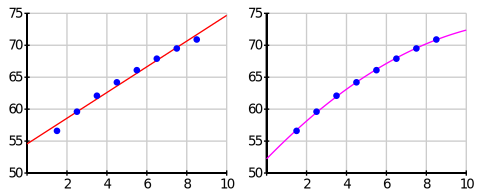
\includegraphics{7_d_least_squares_line}} 
%\resizebox{!}{1.5in}{\includegraphics{least_squares_line}} \hspace{0.2in} \resizebox{!}{1.5in}{\includegraphics{least_squares_quadratic}}
%\end{center}
%\caption{Left: Least squares line. Right: Least squares quadratic.}
%\label{F:LS_linear}
%\end{figure}   
		
%	\item The first date point would satisfy $(1.5^2)a_2+1.5a_1+a_0 = 56.6$, the second $(2.5)^2a_2+2.5a_1+a_0 = 59.6$, and so on, giving us the linear system
%\begin{alignat*}{4}
%{1.5^2}a_2	&{}+{}	&{1.5}a_1	&{}+{}	&a_0 &{}={} 56.6{} \\ 
%{2.5^2}a_2	&{}+{}	&{2.5}a_1	&{}+{}	&a_0 &{}={} 59.6{} \\
%{3.5^2}a_2	&{}+{}	&{3.5}a_1	&{}+{}	&a_0 &{}={} 62.1{} \\
%{4.5^2}a_2	&{}+{}	&{4.5}a_1	&{}+{}	&a_0 &{}={} 64.2{}  \\
%{5.5^2}a_2	&{}+{}	&{5.5}a_1	&{}+{}	&a_0 &{}={} 66.1{} \\
%{6.5^2}a_2	&{}+{}	&{6.5}a_1	&{}+{}	&a_0 &{}={} 67.9{} \\
%{7.5^2}a_2	&{}+{}	&{7.5}a_1	&{}+{}	&a_0 &{}={} 69.5{} \\
%{8.5^2}a_2	&{}+{}	&{8.5}a_1	&{}+{}	&a_0 &{}={} 70.9{.}
%\end{alignat*}
%Letting 
%\[A = \left[ \begin{array}{ccc} 1.5^2&1.5&1 \\ 2.5^2&2.5&1 \\ 3.5^2&3.5&1 \\ 4.5^2&4.5&1 \\ 5.5^2&5.5&1 \\ 6.5^2&6.5&1 \\ 7.5^2&7.5&1 \\ 8.5^2&8.5&1 \end{array} \right], \ \vx = \left[ \begin{array}{c} a_2\\a_1\\a_0 \end{array} \right], \ \text{ and } \ \vb=\left[ \begin{array}{c} 56.6\\59.6\\62.1\\64.2\\66.1\\67.9\\69.5\\70.9 \end{array} \right],\]
%we can write this system in the matrix form  $A \vx = \vb$. 

%Technology shows that every column of the reduced row echelon form of $A$ contains a pivot, so the columns of $A$ are linearly independent. The least squares solution to the system is then found by 
%\[A^+ \vb = (A^{\tr}A)^{-1}A^{\tr} \vb.\]
%Technology shows that (with entries rounded to 3 decimal places) $A^+$ is 
%\[\left[ \arraycolsep=2.5pt  \begin{array}{rrrrrrrr}  0.042& 0.006&- 0.018&- 0.030&- 0.030&- 0.018& 0.006& 0.042\\ - 0.500&- 0.119& 0.143& 0.286& 0.310& 0.214& 0.000&-0.333\\  1.365& 0.540&- 0.049&- 0.403&-0.522&- 0.406&- 0.055& 0.531\end {array} \right],\]
%and 
%\[A^+ \vb \approx \left[ \begin{array}{r} -0.118 \\ 3.195 \\ 52.219 \end{array} \right].\]
%So the least squares quadratic solution to $A\vx = \vb$ is $q$ defined by $q(x) \approx -0.118x^2+3.195x + 52.219$. A graph of $q$ against the data points is shown at right in Figure \ref{F:LS_linear}. 
 	
%	\ea
	

%\end{example}
	

\csection{Summary}
\begin{itemize}
\item The condition number of an $m \times n$ matrix $A$ is the number $||A^{-1}|| \ ||A||$. The condition number provides a measure of how well the relative error in a calculated value $\Delta \vb$ predicts the relative error in $\Delta \vx$ when we are trying to solve a system $A \vx = \vb$.  
\item A pseudoinverse $A^{+}$ of a matrix $A$ can be found through a singular value decomposition. Let $U \Sigma V^{\tr}$ be a singular value decomposition of an $m \times n$ matrix $A$ of rank $r$, with
\[\Sigma = \left[ \begin{array}{ccccc|c} \sigma_1&&&&& \\ & \sigma_2&&0&& \\ && \sigma_3&&&0 \\ & 0 & & \ddots & & \\ &&&& \sigma_r \\ \hline &&0&&&0 \end{array} \right] \]
If $\Sigma^+$ is the $n \times m$ matrix defined by
\[\Sigma^{+} = \left[ \begin{array}{ccccc|c} \frac{1}{\sigma_1}&&&&& \\ & \frac{1}{\sigma_2}&&0&& \\ && \frac{1}{\sigma_3}&&&0 \\ & 0 & & \ddots & & \\ &&&& \frac{1}{\sigma_r} \\ \hline &&0&&&0 \end{array} \right],\]
then $A^{+} = V\Sigma^{+}U^{\tr}$. 
\item A pseudoinverse $A^{+}$ of a matrix $A$ acts like an inverse for $A$. So if we can't solve a matrix equation $A \vx = \vb$ because $\vb$ isn't in $\Col A$, we can use the pseudoinverse of $A$ to ``solve" the equation $A \vx = \vb$ with the ``solution" $A^+ \vb$. While not an exact solution, $A^+ \vb$ turns out to be the best approximation to a solution in the least squares sense. 
%\item If the columns of $A$ are linearly independent, then we can alternatively find the least squares solution as $\left(A^{\tr}A\right)^{-1}A^{\tr}\vb$.
\end{itemize}


\csection{Exercises}
\be
\item Let $A = \left[ \begin{array}{rcc} 20&4&32 \\ -4&4&2 \\ 35&22&26 \end{array} \right]$. Then $A$ has singular value decomposition $U \Sigma V^{\tr}$ , where 
\begin{align*}
U &= \frac{1}{5}\left[ \begin{array}{crc} 3&4&0 \\ 0&0&5 \\ 4&-3&0 \end{array} \right] \\
\Sigma &= \left[ \begin{array}{crc} 60&0&0 \\ 0&15&0 \\ 0&0&6 \end{array} \right] \\
V &= \frac{1}{3}\left[ \begin{array}{crr} 2&-1&-2 \\ 1&-2&2 \\ 2&2&1 \end{array} \right].
\end{align*}
	\ba
	\item What are the singular values of $A$?
	\item Write the outer product decomposition of $A$. 
	\item Find the best rank 1 approximation to $A$. What is the relative error in approximating $A$ by this rank 1 matrix? 
	\item Find the best rank 2 approximation to $A$. What is the relative error in approximating $A$ by this rank 2 matrix?
	\ea

\item Let $A = \left[ \begin{array}{ccrr} 861&3969&70&140 \\ 3969&861&70&140 \\ 3969&861&-70&-140 \\ 861&3969&-70&-140 \end{array} \right]$. 
	\ba
	\item Find a singular value decomposition for $A$. 
	\item What are the singular values of $A$?
	\item Write the outer product decomposition of $A$. 
	\item Find the best rank 1, 2, and 3 approximations to $A$. How much information about $A$ does each of these approximations contain?
	\ea
	
	

%\item The University of Denver Infant Study Center investigated whether babies take longer to learn to crawl in cold months, when they are often bundled in clothes that restrict their movement, than in warmer months. The study sought a relationship between babies' first crawling age and the average temperature during the month they first try to crawl (about 6 months after birth). Some of the data from the study is in Table \ref{T:7_d_infants}. Let $x$ represent the temperature in degrees Fahrenheit and $C(x)$ the average crawling age in months.  

%\begin{table}[h]
%\begin{center}
%\begin{tabular}{|l||c|c|c|c|} \hline
%$x$		&33		&37		&48		&57 \\ \hline
%$C(x)$	&33.83	&33.35	&33.38	&32.32 \\ \hline
%\end{tabular}
%\end{center}
%\caption{Crawling age.}
%\label{T:7_d_infants}
%\end{table}
%	\ba
%	\item Use Theorem \ref{thm:7_d_SVD_cols_lin_indep} to find the least squares line to fit this data. Plot the data and your line on the same set of axes. 
%	\item Use your least squares line to predict the average crawling age when the temperature is 65. 
%	\ea


%\item The cost, in cents, of a first class postage stamp in years from 1981 to 1995 is shown in Table \ref{T:7_d_stamps}.
%\begin{table}[h]
%\begin{center}
%\begin{tabular}{|l||c|c|c|c|c|} \hline
%Year	&1981	&1985	&1988	&1991	&1995 \\ \hline
%Cost	&20		&22		&25		&29		&32  \\ \hline
%\end{tabular}
%\end{center}
%\caption{Cost of postage.}
%\label{T:7_d_stamps}
%\end{table}
%	\ba
%	\item Use Theorem \ref{thm:7_d_SVD_cols_lin_indep} to find the least squares line to fit this data. Plot the data and your line on the same set of axes. 
%	\item Now find the least squares quadratic approximation to this data. Plot the quadratic function on same axes as your linear function. 
%	\item Use your least squares line and quadratic to predict the cost of a postage stamp in this year. Look up the cost of a stamp today and determine how accurate your prediction is. Which function gives a better approximation? Provide reasons for any discrepancies.  
%	\ea

\item Assume that the number of feet traveled by a batted baseball at various angles in degrees (all hit at the same bat speed) is given in Table \ref{T:7_d_batting}.
\begin{table}[h]
\begin{center}
\begin{tabular}{|l||c|c|c|c|c|c|} \hline
Angle			&$10^{\circ}$	&$20^{\circ}$	&$30^{\circ}$	&$40^{\circ}$	&$50^{\circ}$	&$60^{\circ}$ \\ \hline
Distance		&116					&190					&254					&285					&270					&230  \\ \hline
\end{tabular}
\end{center}
\caption{Distance traveled by batted ball.}
\label{T:7_d_batting}
\end{table}
	\ba
	\item Plot the data and explain why a quadratic function is likely a better fit to the data than a linear function.
	\item Find the least squares quadratic approximation to this data. Plot the quadratic function on same axes as your data.
	\item At what angle (or angles), to the nearest degree, must a player bat the ball in order for the ball to travel a distance of 220 feet?
	\ea

%\item Not all data is well modeled with polynomials -- populations tend to grow at rates proportional to the population, which implies exponential growth. For example, Table \ref{T:7_d_US_population} shows the approximate population of the United States in years between 1920 and 2000, with the population measured in millions. 
%\begin{table}[h]
%\begin{center}
%\begin{tabular}{|l||c|c|c|c|c|c|c|c|c|} \hline
%Year			&1920	&1930	&1940	&1950	&1960	&1970	&1980	&1990	&2000 \\ \hline
%Population	&106		&123		&142		&161		&189		&213		&237		&259		&291  \\ \hline
%\end{tabular}
%\end{center}
%\caption{U.S. population.}
%\label{T:7_d_US_population}
%\end{table}
%If we assume the population grows exponentially, we would want to find the best fit function $f$ of the form $f(t) = ae^{kt}$, where $a$ and $k$ are constants. To apply the methods we have developed, we could instead apply the natural logarithm to both sides of $y = ae^{kt}$ to obtain the equation $\ln(y) = \ln(a) + kt$. We can then find the best fit line to the data in the form $(t, \ln(y))$ to determine the values of $\ln(a)$ and $k$. Use this approach to find the best fit exponential function in the least squares sense to the U.S. population data.

\item How close can a matrix be to being non-invertible? We explore that idea in this exercise. Let $A = [a_{ij}]$ be the $n \times n$ upper triangular matrix with 1s along the diagonal and with every other entry being $-1$. 
	\ba
	\item What is $\det(A)$? What are the eigenvalues of $A$? Is $A$ invertible?  


	\item Let $B = [b_{ij}]$ be the $n \times n$ matrix so that $b_{n1} = -\frac{1}{2^{n-2}}$ and $b_{ij} = a_{ij}$ for all other $i$ and $j$. 
		\begin{enumerate}[i.]
		\item For the matrix $B$ with $n=3$, show that the equation $B \vx = \vzero$ has a non-trivial solution. Find one non-trivial solution. 
	
		\item For the matrix $B$ with $n=4$, show that the equation $B \vx = \vzero$ has a non-trivial solution. Find one non-trivial solution. 
	

		\item Use the pattern established in parts (i.) and (ii.) to find a non-trivial solution to the equation $B \vx = \vzero$ for an arbitrary value of $n$. Be sure to verify that you have a solution. Is $B$ invertible? (Hint: For any positive integer $m$, the sum  $1+\sum_{k=0}^{m-1} 2^k$ is the partial sum of a geometric series with ratio $2$ and so $1+\sum_{k=0}^{m-1} 2^k  = 1+\frac{1-2^m}{1-2} = 2^m$.)

		\item Explain why $B$ is not an invertible matrix. Notice that $A$ and $B$ differ by a single entry, and that $A$ is invertible and $B$ is not. Let us examine how close $A$ is to $B$. Calculate $|| A - B ||_F$? What happens to $||A - B||_F$ as $n$ goes to infinity? How close can an invertible matrix be to becoming non-invertible? 

		\end{enumerate}

	\ea
 
 \item Let $A = \left[ \begin{array}{crr} 1&0&0 \\ 0&1&-1 \\ 0&-1&1 \end{array} \right]$. In this exercise we find a matrix $B$ so that $B^2 = A$, that is, find a square root of the matrix $A$. 
	\ba
	\item Find the eigenvalues and corresponding eigenvectors for $A$ and $A^{\tr}A$. Explain what you see. 
	
	\item Find a matrix $V$ that orthogonally diagonalizes $A^{\tr}A$. 
	
\item Exercise \ref{ex:7_c_Symmetric_SVD} in Section \ref{sec:SVD} shows if $U \Sigma V^{\tr}$ is a singular value decomposition for a symmetric matrix $A$, then so is $V \Sigma V^{\tr}$. Recall that $A^n = \left(V \Sigma V^{\tr}\right)^n = V \Sigma^n V^{\tr}$ for any positive integer $n$. We can exploit this idea to define $\sqrt{A}$ to be the matrix
	\[V \Sigma^{1/2}V^{\tr},\]
	where $\Sigma^{1/2}$ is the matrix whose diagonal entries are the square roots of the corresponding entries of $\Sigma$. Let $B = \sqrt{A}$. Calculate $B$ and show that $B^2 = A$. 

	\item Why was it important that $A$ be a symmetric matrix for this process to work, and what had to be true about the eigenvalues of $A$ for this to work? 
	
	\item Can you extend the process in this exercise to find a cube root of $A$? 
	
	\ea


\item Let $A$ be an $m \times n$ matrix with singular value decomposition $U \Sigma V^{\tr}$. Let $A^{+}$ be defined as in (\ref{eq:pseudoinverse}). In this exercise we prove the remaining parts of Theorem \ref{thm:7_d_pseudoinverse}.
	\ba
	\item Show that $(AA^{+})^{\tr} = AA^{+}$. (Hint: $\Sigma \Sigma^+$ is a symmetric matrix.)

	
	\item Show that $(A^{+}A)^{\tr} = A^{+}A$. 

	\ea

\item In this exercise we show that the pseudoinverse of a matrix is the unique matrix that satisfies the Moore-Penrose conditions. Let $A$ be an $m \times n$ matrix with singular value decomposition $U \Sigma V^{\tr}$ and pseudoinverse $X = V\Sigma^{+}U^{\tr}$. To show that $A^{+}$ is the unique matrix that satisfies the Moore-Penrose conditions, suppose that there is another matrix $Y$ that also satisfies the Moore-Penrose conditions. 
	\ba
	\item Show that $X = YAX$. 
	
	\item Show that $Y = YAX$. 

	\item How do the results of parts (a) and (b) show that $A^{+}$ is the unique matrix satisfying the Moore-Penrose conditions?


	\ea
	
\item Find the pseudoinverse of the $m \times n$ zero matrix $A=0$. Explain the conclusion.

\item In all of the examples that we have done finding a singular value decomposition of a matrix, it has been the case (though we haven't mentioned it), that if $A$ is an $m \times n$ matrix, then $\rank(A) = \rank\left(A^{\tr}A\right)$. Prove this result.

	
\item Label each of the following statements as True or False. Provide justification for your response.
	\ba
	\item \textbf{True/False} A matrix has a pseudo-inverse if and only if the matrix is singular. 
	\item \textbf{True/False} The pseudoinverse of an invertible matrix $A$ is the matrix $A^{-1}$. 
	\item \textbf{True/False} If the columns of $A$ are linearly dependent, then there is no least squares solution to $A\vx = \vb$. 
	\item \textbf{True/False} If the columns of $A$ are linearly independent, then there is a unique least squares solution to $A\vx = \vb$.
	\item \textbf{True/False} If $T$ is the matrix transformation defined by a matrix $A$ and $S$ is the matrix transformation defined by $A^{+}$, then $T$ and $S$ are inverse transformations. 
	\ea


\ee

\csection{Project: GPS and Least Squares}

In this project we discuss some of the details about how the GPS works. The idea is based on intersections of spheres. To build a basic understanding of the system, we begin with a 2-dimensional example. 

\begin{pactivity} \label{act:GPS_plane_ex} Suppose that there are three base stations $A$, $B$,  and $C$ in $\R^2$ that can send and receive signals from your mobile phone. Assume that $A$ is located at point $(-1,-2)$, $B$ at point $(36,5)$, and $C$ at point $(16,35)$. Also assume that your mobile phone location is point $(x,y)$. Based on the time that it takes to receive the signals from the three base stations, it can be determined that your distance to base station $A$ is $28$ km, your distance to base station $B$ is $26$ km, and your distance to base station $C$ is $14$ km using a coordinate system with measurements in kilometers based on a reference point chosen to be $(0,0)$. Due to limitations on the measurement equipment, these measurements all contain some unknown error which we will denote as $z$. The goal is to determine your location in $\R^2$ based on this information.

If the distance readings were accurate, then the point $(x,y)$ would lie on the circle centered at $A$ of radius $29$. The distance from $(x,y)$ to base station $A$ can be represented in two different ways: $28$ km and $\sqrt{(x+1)^2 + (y+2)^2}$. However, there is some error in the measurements (due to the receiver clock and satellite clocks not being snychronized), so we really have 
\[\sqrt{(x+1)^2 + (y+2)^2} + z = 28,\]
where $z$ is the error.
Similarly, $(x,y)$ must also satisfy 
\[\sqrt{(x-36)^2 + (y-5)^2} + z = 26\]
and
\[\sqrt{(x-16)^2 + (y-35)^2} + z = 14.\]

\ba
\item Explain how these three equations can be written in the equivalent form
\begin{align}
(x+1)^2+(y+2)^2&=(28-z)^2 \label{eq:GPS_2D_1} \\
(x-36)^2 + (y-5)^2 &= (26-z)^2 \label{eq:GPS_2D_2} \\
(x-16)^2 + (y-35)^2 &= (14-z)^2. \label{eq:GPS_2D_3}
\end{align}


\begin{figure}[h]
\begin{center}
\resizebox{!}{1.5in}{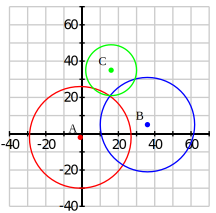
\includegraphics{7_d_Ex2_D_circles}} 
\caption{Intersections of circles.}
\label{F:GPS_circles}
\end{center}
\end{figure}

\item If all measurements were accurate, your position would be at the intersection of the circles centered at $A$ with radius $28$ km, centered at $B$ with radius $26$ km, and centered at $C$ with radius $14$ km as shown in Figure \ref{F:GPS_circles}. Even though the figure might seem to imply it, because of the error in the measurements the three circles do not intersect in one point. So instead, we want to find the best estimate of a point of intersection that we can. The system of equations \ref{eq:GPS_2D_1}, \ref{eq:GPS_2D_2}, and \ref{eq:GPS_2D_3} is non-linear and can be difficult to solve, if it even has a solution. To approximate a solution, we can linearize the system. To do this, show that if we subtract corresponding sides of equation  (\ref{eq:GPS_2D_1}) from (\ref{eq:GPS_2D_2}) and expand both sides, we can obtain the linear equation
\[37x + 7y + 2z = 712\]
in the unknowns $x$, $y$, and $z$. 

\item Repeat the process in part (b), subtracting (\ref{eq:GPS_2D_1}) from (\ref{eq:GPS_2D_3}) and show that we can obtain the linear equation
\[17x + 37y + 14z = 1032\]
in $x$, $y$, and $z$.

\item We have reduced our system of three non-linear equations to the system
\begin{alignat*}{4}
{37}x 	&{}+{} 	&{7}y 	&{}+{}	&{2}z 	&= &{} 	&712\\
{17}x		&{}+{} 	&{37}y 	&{}+{} 	&{14}z	&= &{}	&1032
\end{alignat*} 
of two linear equations in the unknowns $x$, $y$, and $z$. Use technology to find a pseudoinverse of the coefficient matrix of this system. Use the pseudoinverse to find the least squares solution to this system. Does your solution correspond to an approximate point of intersection of the three circles? 

\ea

\end{pactivity}

Project Activity \ref{act:GPS_plane_ex} provides the basic idea behind GPS. Suppose you receive a signal from a GPS satellite. The transmission from satellite $i$ provides four pieces of information --  a location $(x_i,y_i,z_i)$ and a time stamp $t_i$ according to the satellite's atomic clock. The time stamp allows the calculation of the distance between you and the $i$th satellite. The transmission travel time is calculated by subtracting the current time on the GPS receiver from the satellite's time stamp. Distance is then found by multiplying the transmission travel time by the rate, which is the speed of light $c=299792.458$ km/s.\footnote{The signals travel in radio waves, which are electromagnetic waves, and travel at the speed of light. Also, $c$ is the speed of light in a vacuum, but atmosphere is not too dense so we assume this value of $c$} So distance is found as $c(t_i-d)$, where $d$ is the time at the receiver. This signal places your location within in a sphere of that radius from the center of the satellite. If you receive a signal at the same time from two satellites, then your position is at the intersection of two spheres. As can be seen at left in Figure \ref{F:Spheres}, that intersection is a circle. So your position has been narrowed quite a bit. Now if you receive simultaneous signals from three spheres, your position is narrowed to the intersection of three spheres, or two points as shown at right in Figure \ref{F:Spheres}.  So if we could receive perfect information from three satellites, then your location would be exactly determined.
\begin{figure}[h]
\begin{center}
\resizebox{!}{2.0in}{\includegraphics{7_d_two_spheres.jpg}} \hspace{0.5in} \resizebox{!}{2.0in}{\includegraphics{7_d_three_spheres.jpg}}
%\resizebox{!}{1.5in}{\includegraphics[trim=0.4cm 0.4cm 1.1cm 1.4cm, clip]{two_spheres.png}} \hspace{0.5in} \resizebox{!}{1.5in}{\includegraphics[trim=0.4cm 0.4cm 1.1cm 0.9cm, clip]{three_spheres.png}}
\caption{Intersections of spheres.}
\label{F:Spheres}
\end{center}
\end{figure}
%crop graphics in animate trim=<left> <bottom> <right> <top>, clip with includegraphics

There is a problem with the above analysis -- calculating the distances. These distances are determined by the time it takes for the signal to travel from the satellite to the GPS receiver. The times are measured by the clocks in the satellites and the clocks in the receivers. Since the GPS receiver clock is unlikely to be perfectly synchronized with the satellite clock, the distance calculations are not perfect. In addition, the rate at which the signal travels can change as the signal moves through the ionosphere and the troposphere. As a result, the calculated distance measurements are not exact, and are referred to as \emph{pseudoranges}. In our calculations we need to factor in the error related to the time discrepancy and other factors. We will incorporate these errors into our measure of $d$ and treat $d$ as an unknown. (Of course, this is all more complicated that is presented here, but this provides the general idea.) 

To ensure accuracy, the GPS uses signals from four satellites. Assume a satellite is positioned at point $(x_1,y_1,z_1)$ at a distance $d_1$ from the GPS receiver located at point $(x,y,z)$. The distance can also be measured in two ways: as 
\[\sqrt{(x-x_1)^2+(y-y_1)^2+(z-z_1)^2}.\]
and as $c(t_1-d)$. So 
\[c(t_1-d) = \sqrt{(x-x_1)^2 + (y-y_1)^2 + (z-z_1)^2}.\]
Again, we are treating $d$ as an unknown, so this equation has the four unknowns $x$, $y$, $z$, and $d$. Using signals from four satellites produces the system of equations
\begin{align}
\sqrt{(x-x_1)^2 + (y-y_1)^2 + (z-z_1)^2} &=  c(t_1-d)  \label{eq:GPS_1_sqrt} \\
\sqrt{(x-x_2)^2 + (y-y_2)^2 + (z-z_2)^2}  &=  c(t_2-d)  \label{eq:GPS_2_sqrt} \\
\sqrt{(x-x_3)^2 + (y-y_3)^2 + (z-z_3)^2} &=  c(t_3-d)  \label{eq:GPS_3_sqrt} \\
\sqrt{(x-x_4)^2 + (y-y_4)^2 + (z-z_4)^2} &=  c(t_4-d). \label{eq:GPS_4_sqrt}
\end{align}


\begin{pactivity} \label{act:GPS_3D} The system of equations (\ref{eq:GPS_1_sqrt}), (\ref{eq:GPS_2_sqrt}), (\ref{eq:GPS_3_sqrt}), and (\ref{eq:GPS_4_sqrt}) is a non-linear system and is difficult to solve, if it even has a solution. We want a method that will provide at least an approximate solution as well as apply if we use more than four satellites. We choose a reference node (say $(x_1, y_1, z_1)$) and make calculations relative to that node as we did in Project Activity \ref{act:GPS_plane_ex}.
\ba
\item First square both sides of the equations (\ref{eq:GPS_1_sqrt}), (\ref{eq:GPS_2_sqrt}), (\ref{eq:GPS_3_sqrt}), and (\ref{eq:GPS_4_sqrt}) to remove the roots. Then subtract corresponding sides of the new first equation (involving $(x_1,y_1,z_1)$) from the new second equation  (involving $(x_2,y_2,z_2)$) to show that we can obtain the linear equation 
\[2(x_2-x_1)x + 2(y_2-y_1)y + 2(z_2-z_1)z + 2c^2(t_1-t_2)d = c^2(t_1^2-t_2^2)  - h_1 +h_2,\]
where $h_i = x_i^2 + y_i^2 + z_i^2$. (Note that the unknowns are $x$, $y$, $z$, and $d$ -- all other quantities are known.)

\item Use the result of part (a) to write a linear system that can be obtained by subtracting the first equation from the third and fourth equations as well. 

\item The linearizations from part (b) determine a system $A \vx = \vb$ of linear equations. Identify $A$, $\vx$, and $\vb$. Then explain how we can approximate a best solution to this system in the least squares sense. 

\ea

\end{pactivity}

We conclude this project with a final note. At times a GPS receiver may only be able to receive signals from three satellites. In these situations, the receiver can substitute the surface of the Earth as a fourth sphere and continue the computation. 	



